



Flow in the sanitary sewer network can be classified as Dry-Weather Flow (DWF) and Wet-Weather Flow (WWF). DWF can be further divided in two components: 1. Base Waste Flow (BWF): inflow of waste water coming from households, commercial and industrial sites; and 2. Groundwater Infiltration (GWI): Water from aquifers that infiltrates into the network thought defects such as pipe cracks and leaky joints(Vallabhaneni and Burgess 2007). 
The choice of the hydrological model in this study aims the representation of RDII, which is the incremental flow into the sanitary sewer system caused by precipitation (rainfall or snowmelt). Figure 3 shows the typical characteristics of different components of sanitary sewer flow. RDII needs to be first separated from DWF when processing raw data coming from flow meters. More about the methods to separate the components are discussed on section 4.2.


\begin{figure}[ht]
    \centering
	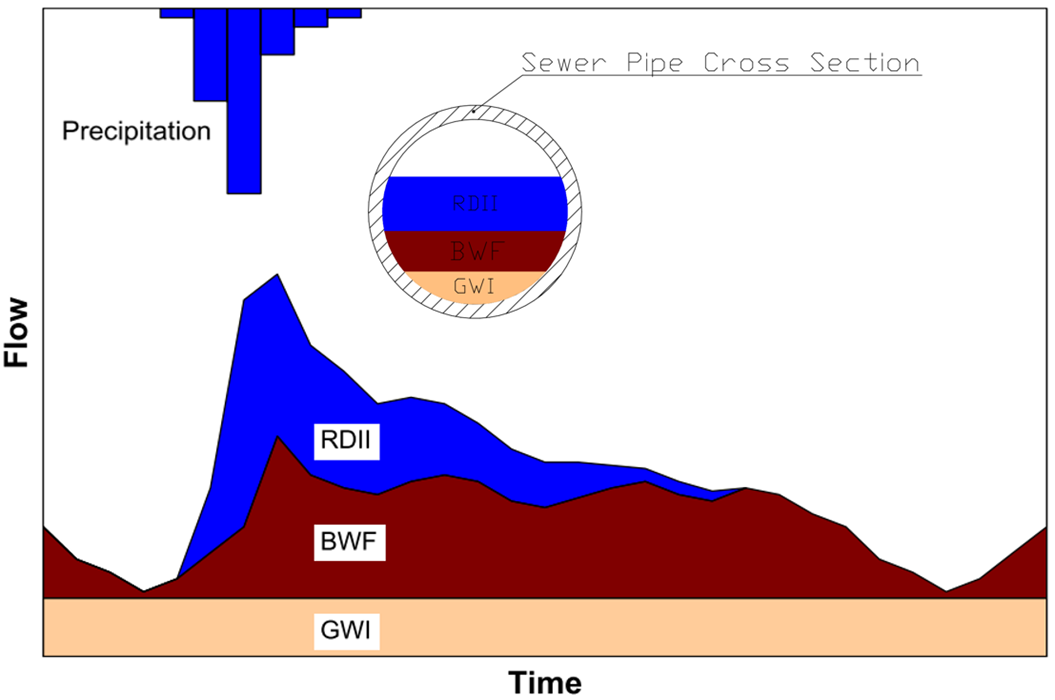
\includegraphics[scale=0.6]{figures/RDII_flows.png}
	\caption{Wet-weather flow components. Modified from \cite{Vallabhaneni2007}}
	\label{fig:flowcomponents}
\end{figure}


\begin{figure}[ht]
    \centering
	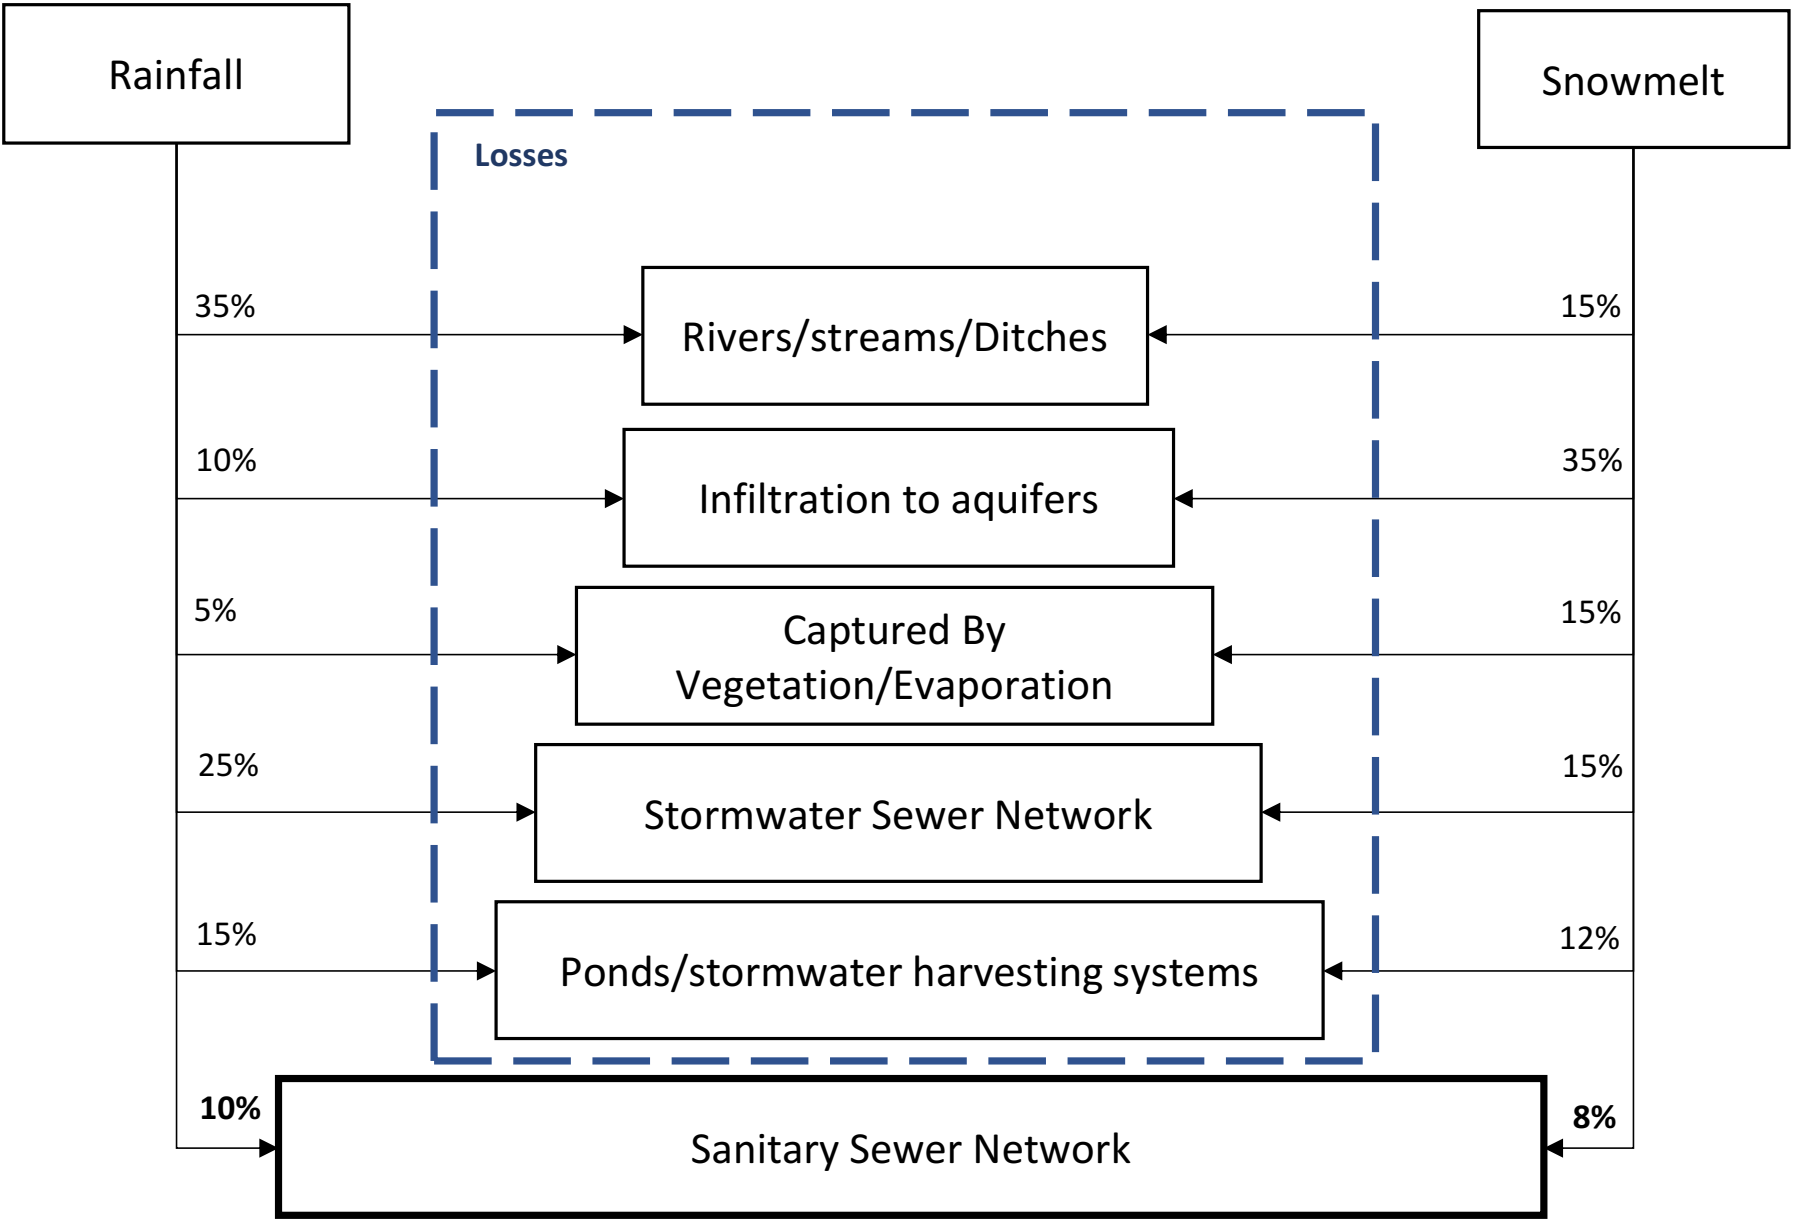
\includegraphics[scale=0.4]{figures/losses.png}
	\caption{Precipitation Losses relative to a Sanitary Sewer Network}
	\label{fig:losses}
\end{figure}

\section{Methods to Quantify Rainfall Dependent Infiltration and Inflow}


As mentioned on section 1. There are different ways stormwater or snowmelt finds its way into the sanitary sewer lines which ideally would have only wastewater from urban developments such as households, commercial centers, factories, etc.  Sanitary sewer networks’ flow increase can be trigged by an event such as a storm or elevation of the groundwater table. From rainfall or snowmelt water flows over the soil surface and inflows to the sanitary sewer through manhole leaky covers or directly from roof-drain and foundation connections. The flow increases in the sanitary sewer due to inflow is generally observed few hours after the beginning of the storm or snowmelt. As depicted in figure X, rainfall or snowmelt   Once the water infiltrates, it moves through the soil porous with a much slower velocity due to the characteristics of the groundwater flow. Infiltration of groundwater flow which reaches the elevation of pipe. Direct roof drain connections. Groundwater infiltration from saturated soil.   
There are many processes where. Function of the infiltration, groundwater flow, surface runoff, flow through pipe fissures.

Rainfall dependent infiltration and inflow have been modeled with different methods. Bennet (1999) (Bennett et al. 1999) carried a literature review and case study of around 10 different methods for quantifying RDII. 
The study concluded that only the regression and unit hydrograph methods are suitable when applying continuous simulation for long-term modelling. The unit hydrograph (UH) method also provided the best consistent match to storm peaks. Vallabhaneni and Burguess (2007) (Vallabhaneni and Burgess 2007) and U.S. EPA (2008) (Epa et al. n.d.) also considered sewer network rehabilitation capabilities as a factor for evaluation of the methods and suggested that regression should be used when more than 2 years of recorded flow and rainfall data is available. When no flow is available, the Constant Unit Rate RDII Method seems to be useful since it accounts for spatial characteristics of the Sewershed and information of pipe characteristics and population. Moreover, U.S. EPA (2008) study concluded that Unit Hydrograph RTK method can be useful to identify if which portion of the wet-weather flow is caused by inflow and which portion is caused by infiltration. Knowing whether RDII is more impacted by inflow or infiltration is relevant when evaluating the sanitary sewer network for rehabilitation. 
It is important to mention that the studies also concluded that there is no RDII quantification method that can be universally applied, since their use depend on available data and characteristics of the catchment. The goal of Vallabhaneni and Burguess (2007) (Vallabhaneni and Burgess 2007) and U.S. EPA (2008) (Epa et al. n.d.) reviews were to choose the most suitable method to be first implemented in a toolbox named as Sanitary Sewer Overflow Analysis and Planning (SSOAP). 




TELL HERE WHY THE CHOICE OF RDII AND SWMM

As described in section X. Two main reasons was to model snowmelt was the primary motivation to use SWMM modules and subcatchments in this study. and a model that could simulate the watershed behaviour throuout all the seasons of the year. 

\section{Physically-Based: SWMM Modules}

The use of SWMM packages in this study aimed to model four processes happening simultaneously in the watershed to simulate fast, medium and long term response observed in \ac{SSN} wet-weather flows. The four processes/SWMM modules are described here as: 1. Runoff; 2. Snowpack \& Snowmelt; 3. Infiltration; 4. Groundwater. 

%=======================================================================
% RAINFALL-RUNOFF
%=======================================================================

\subsection{Rainfall-Runoff} 

%=======================================================================
% SNOWPACK AND SNOWMELT
%=======================================================================

\subsection{Snowpack \& Snowmelt} \label{snowlit}

Snowpack \& snowmelt module was used to simulate the variations of flows in the \acf{SSN} occurring during winter conditions since a considerable incremental quantity of infiltration occurs during snowmelt periods as showed on the available data of section \ref{flowdata}.

Snowpack \& snowmelt calculation routines available in SWMM were based on models developed by \acf{NWS} \cite{anderson1973,anderson2006}. SWMM models the depth of water equivalent as the snowpack. The depth is increased during snow accumulation periods and decreased when snowmelt occurs. The amount of water released from the snowpack during snowmelt is transformed in precipitation rate [mm/h] and summed to the rainfall as "net precipitation" that is used as input to compute surface runoff. Therefore, snowmelt calculations are part of runoff module \cite{Rossman2016}.

Three of the key parameters for snowmelt routine are:
\begin{enumerate}
    \item $T_a$: air temperature of the current time step [C°]
    \item $T_{base}$: The base temperature of which snowmelt starts to occur [C°]
    \item $DHM$: melt coefficient [mm/h/C°]
\end{enumerate}

These three parameters are used in the linear type equation \ref{eqn:smeltdry} to compute the snowmelt [mm/h] during dry periods. Calculations of snowmelt during wet periods (greater than 0.51 mm/h) take also in consideration the wind speed and local atmospheric pressure. Refer to \citet{anderson1973,anderson2006} or \citet{Rossman2016} for detailed description of snowmelt calculations during rainfall.

\begin{equation}
\label{eqn:smeltdry}
SMELT = DHM \cdot (T_a - T_{base}) 
\end{equation}

Melt coefficient ($DHM$) varies seasonally and is calculated based on a sinusoidal equation and two user-supplied constants: 1. Minimum melt coefficient ($DHM_{min}$) which happens on December 21\textsuperscript{th}; 2. Maximum melt ($DHM_{max}$) happening on June 21\textsuperscript{th} as depicted in figure \ref{fig:meltcoeff}. 

\begin{figure}[h]
    \centering
	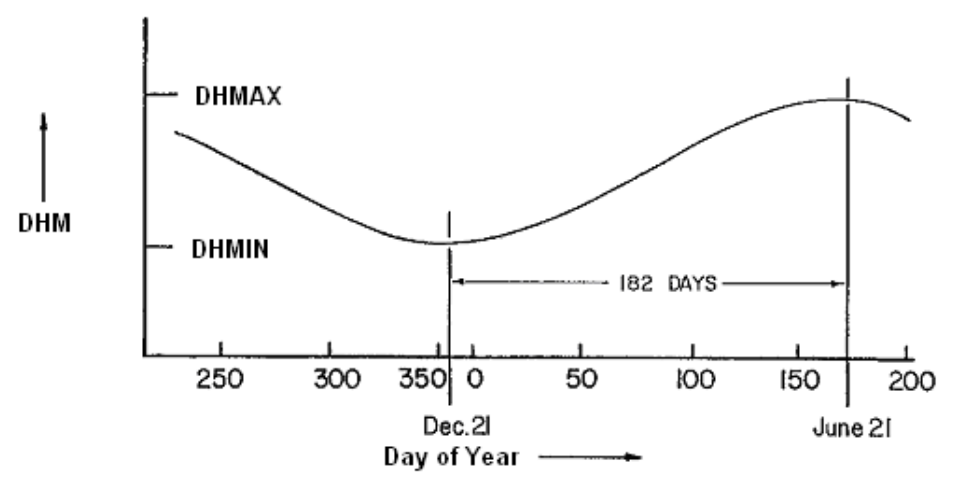
\includegraphics[scale=0.55]{figures/snowmelt_DHM.png}
	\caption{Seasonal variation of melt coefficients \cite{Rossman2016}}
	\label{fig:meltcoeff}
\end{figure}

 Before snowmelt occurs, the snowpack status has to be assessed. For this, there are two condition:
 \begin{enumerate}
    \item The snowpack has to be heated with air temperatures higher than $T_{base}$.
    \item Snowmelt has to fill the voids within the snowpack. Meaning that there is a quantity of water contained in the snowpack and it is considered to be a fraction of the "depth of water equivalent" and named as fraction of free water capacity ($FWC$). 
\end{enumerate}
  
The heat content in the pack is calculated and $FWC$ a user-supplied value. Therefore, liquid melt will only become a component of "net precipitation" after the two conditions, above mentioned, are satisfied.

 The difference between heat content of the snowpack and $T_{base}$ is named as "cold content" ($COLDC$). This variable is used to compute how much heat is necessary to be transfered to the snowpack before snowmelt can occur, as the first condition metioned above. The $COLDC$ value is updated every time step based on the heat transfer between the pack and the atmosphere. The variation of the cold content ($\Delta CC$) is calculated every time step assuming a negative value during melting periods. The following two user-supplied constant fractions are necessary to compute $\Delta CC$:
\begin{enumerate}
    \item $RNM$: Negative melt ratio [fraction]
    \item $TIPM$: ATI weight ratio [fraction]
\end{enumerate}

The rate of which heat transfer occurs is calculated based on SWMM's internal parameter of antecedent temperature index ($ATI$) which is function of $T_a$ and $TIPM$. Values of $TIPM$ towards tending to zero represent a thicker pack which warms and cools slowly as a greater weight is given to more antecedent temperatures. Equation \ref{eqn:ddcdry} is used when $T_a$ < $T_{base}$ and equation \ref{eqn:ddcwet} when $T_a$ > $T_{base}$ \cite{Rossman2016}. 

\begin{equation}
\label{eqn:ddcdry}
\Delta CC = RNM \cdot DHM \cdot (ATI - T_a) \cdot Time Step
\end{equation}

\begin{equation}
\label{eqn:ddcwet}
\Delta CC = - SNOWMELT \cdot RNM \cdot Time Step
\end{equation}

The Negative Melt Ratio ($RNM$) in equations \ref{eqn:ddcdry} and \ref{eqn:ddcwet} is used to account for a reduced heat transfer during periods without "actual liquid melt".
Snow plowing and areal depletion were not used in this study for lack of data and simplicity.
Other three parameters used were:

\begin{enumerate}
    \item $U$: Monthly average wind speed [m/s]
    \item $Z_{el}$: elevation above mean sea level [m]
    \item $SNOTMP$: Dividing temperature between snowfall and rainfall [C°]
    \item $SCF$: Snow catch factor [ratio]
\end{enumerate}

Where 1. and 2. were used to compute the influence of wind speed on the melting of snow during rainfall periods and 3. and 4. used to define the amount of snowfall from raw precipitation input data.


%Snow plowing routine was not utilized in this study for three reasons: 1. No data of snow plowing routines were assessed for the study area; 2. Assumption of no transport of snow among subcatchments; 3. Plowing of snow from impervious to pervious areas within the subcatchment assumed to be negligible since snowmelt can be routed to the pervious areas within SWMM's runoff module.

Table \ref{tbl:snowparam} depict all parameters used for the snowpack \& snowmelt module in this study and their proposed range based on other study cases available in the literature. 


\begin{table}[h]
\caption{Snowpack \& Snowmelt parameters range\cite{Rossman2016}}
\label{tbl:snowparam}
\centering
\begin{tabular}{lcc}
\toprule
\textbf{Parameter}                                                                                                           & \textbf{Proposed Range}                      & \textbf{Units}                     \\ \hline
SNOTMP                                                                                                                       & 0 - 2                                        & {[}°C{]}                           \\
SCF                                                                                                                          & 1 - 2                                     & {[}1{]}                            \\
T\textsubscript{base}                                                                                       & -4 - 0                                       & {[}°C{]}                           \\
\begin{tabular}[c]{@{}l@{}}DHM\textsubscript{min - max} \end{tabular} & 0.019 - 0.11                                 & {[}mm/°C-h{]}                      \\
RNM                                                                                                                          & 0 - 1                                        & {[}1{]}                            \\
FWFRAC                                                                                                                       & 0.01 - 0.25                                   & {[}1{]}                            \\
TIPM                                                                                                                         & 0 - 1                                        & {[}1{]}                            \\
T\textsubscript{a}; Z\textsubscript{el}; $U$                                               & \multicolumn{2}{c}{Location Based (see section \ref{meteodata})}
\end{tabular}
\end{table}

RNM and TIPM bare the full possible range. However, suggestions available in the literature were used as initial values in this study. All other ranges of parameters in \ref{tbl:snowparam}, exept by $DHM_{min - max}$, were proposed as suggested by \citeauthor{Rossman2016} \citeyearpar{Rossman2016} in the SWMM hydrology reference manual \cite{Rossman2016}.

\citeauthor{Tikkanen2013} \citeyearpar{Tikkanen2013} suggested values for the degree-hour melt coefficients ($DHM_{min - max}$) when modelling a catchment in Finland based on values calibrated by \citeauthor{valeo2004} \citeyearpar{valeo2004} for a catchment in Calgari, Canada. \citeauthor{Tikkanen2013} used reduced values in comparison to \citeauthor{valeo2004} to account for fewer solar radiation due to difference in latitude. \citeauthor{valeo2004} calibrated different values of $DHM_{min - max}$ for snow covered pervious and impervious areas varying from 0.02 for $DHM_{min}$ to 0.150 $DHM_{max}$. Therefore, the proposed range in this study was based on \citeauthor{Tikkanen2013} and \citeauthor{valeo2004} findings.

%=======================================================================
% INFILTRATION
%=======================================================================

\subsection{Infiltration} \label{infiltration}

An infiltration model was used in this study to assess long-term simulations (up to 6 months) of the winter periods using snowmelt routine. As \acf{GWI} is one of the components of \acf{SSN} flows, an aquifer and groundwater inflow models were included. The gradient of groundwater infiltration to the \ac{SSN} is dependent on the water table elevation (see section \ref{groundwater}). Therefore, the infiltration routine was included as a way to recharge the modeled aquifer varying the saturated zone elevation (water table) providing a connection between effective precipitation and the \ac{GWI} component.

SWMM version 5.1 package offers the modeller five different infiltration models. The Modified Horton method \cite{akan1992,akan2003} was chosen among the options for three main reasons: 1. it is simply one of the default methods available in SWMM;  2. it has the same parameters as the well-known Horton method which parameter estimates are suggested in \citet{Rossman2016}; 3. Appears to be more accurate low intensity rainfall events than the original Horton method \cite{Rossman2016}. 

The two governing equations of the method describes the infiltration capacity decay during wet periods \ref{eqn:mhortondecay} and its recovery curve during dry periods \ref{eqn:mhortonrecoveryintegrated} and an example of these two curves and how the infiltration capacity would change over time is plotted in figure \ref{fig:horton}. 

\begin{figure}[h]
    \centering
	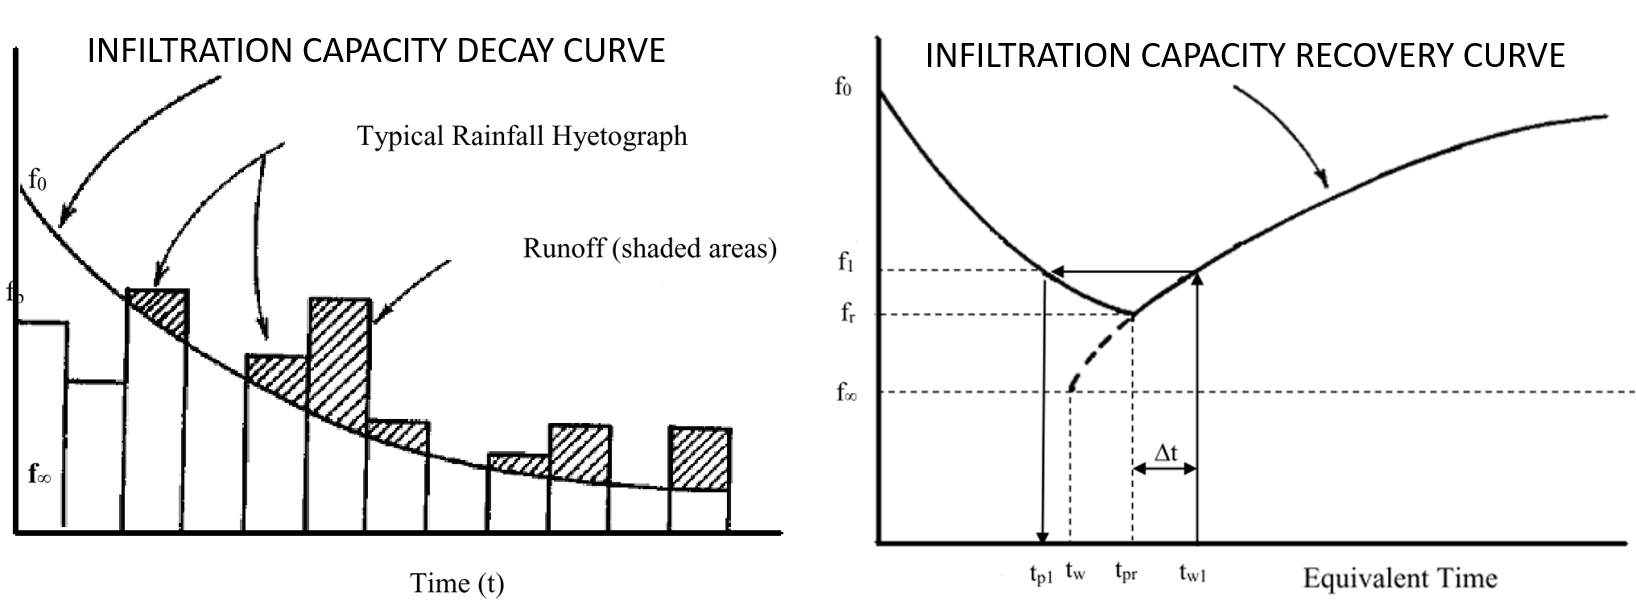
\includegraphics[scale=0.45]{figures/hortoncurves.png}
	\caption{Horton infiltration capacity decay and recovery curves. Modified from \cite{Rossman2016}}
	\label{fig:horton}
\end{figure}

\begin{equation}
\label{eqn:mhortondecay}
F = f_\infty \cdot t + \frac{(f_0 - f_\infty)}{k_d} \cdot (1 - e^{-k_d\cdot t})
\end{equation}
Where: \\
\indent $F$ = cumulative infiltration capacity [ft] \\
\indent $f_\infty$ = minimum or equilibrium value of infiltration capacity at $t = \infty$  [ft/sec] \\
\indent $f_0$ = maximum or initial value of infiltration capacity at $t = 0$ [ft/sec] \\
\indent $t$ = equivalent time [sec] \\
\indent $k_d$ = decay coefficient [sec\textsuperscript{-1}] \\

It is worth to mention that \ref{eqn:mhortondecay} is an integrated form of Horton's original equation. SWMM uses integrated form to consider the intensity of the rainfall event also as a function of the infiltration capacity reduction \cite{Rossman2016}. 


\begin{equation}
\label{eqn:mhortonrecovery}
\frac{df_r}{dt} = kr \cdot (f_0 - f_r) 
\end{equation}
Where: \\

\indent $f_r$ = infiltration capacity during recovery [ft] \\
\indent $f_{r0}$ = maximum or initial value of infiltration capacity at $t = 0$ [ft/sec] \\
\indent $k_r$ = regeneration coefficient [1/sec] \\
\indent $t$ = time [sec] \\

the infiltration capacity at time $t$ after integrating \ref{eqn:mhortonrecovery} when infiltration capacity is $f_{r0}$ is:

\begin{equation}
\label{eqn:mhortonrecoveryintegrated}
f_r =  f_0 - (f_0 - f_{r0}) \cdot e^{-k_d \cdot t}
\end{equation}
    
SWMM computation scheme first checks for wet-period (rainfall/snowmelt) or dry period to apply either of the equations \ref{eqn:mhortondecay} or \ref{eqn:mhortonrecoveryintegrated}  and compute the current infiltration capacity and the amount of water infiltrating the soil. More details of the equations and computational scheme are available in \citet{Rossman2016}.

Table \ref{tbl:infparam} presents a rough estimate of the range of four input parameters for Horton infiltration model. The range was extracted from EPA SWMM user help. 
 

\begin{table}[h]
\caption{Modified Horton infiltration parameters range\cite{Rossman2016}}
\label{tbl:infparam}
\centering
\begin{tabular}{@{}lcll@{}}
\toprule
\textbf{Parameter}        & \multicolumn{2}{c}{\textbf{Typical Range}} & \textbf{Units}        \\ \midrule
Maximum infiltration rate & \multicolumn{2}{c}{8.5 - 254}              & mm/h                  \\
Minimum infiltration rate & \multicolumn{2}{c}{0.254 - 120.4}          & mm/h                  \\
Decay coefficient         & \multicolumn{2}{c}{2 - 7}                  & h\textsuperscript{-1}\\
Drying Time               & \multicolumn{2}{c}{2 - 14}                 & days                  \\ \bottomrule
\end{tabular}
\end{table}


%=======================================================================
% AQUIFER AND GROUNDWATER
%=======================================================================

\subsection{Aquifer \& Groundwater Flow} \label{groundwater}
 
choice of groundwater flow equation:


\section{Synthetic Unit Hydrograph: RTK}





